\subsection*{Partie A}

\begin{enumerate}
	\item Le nombre $x$ représente le nombre de filles ayant obtenu le bac STMG en 2020
	sans mention ou avec la mention assez bien.

\[x = 52 - 13 = 39.\]

	\item La personne est choisie au hasard : on est en situation d'équiprobabilité.
	\begin{enumerate}
		\item La probabilité qu'il s'agisse d'un garçon est égale à $\dfrac{48}{100} = 0,48$.

		\item La probabilité qu'il s'agisse d'une fille ayant obtenu la mention B ou TB est égale à
		$\dfrac{13}{100} = 0,13$.
	\end{enumerate}

	\item Parmi les 52 filles, 13 ont obtenu la mention B ou TB :
	\[\dfrac{13}{52} = \dfrac{13\times 1}{13 \times 4} = \dfrac{1}{4} = 0,25.\]
	L'affirmation est vraie.
\end{enumerate}

\subsection*{Partie B}

La probabilité de choisir une fille est $0,1$ et celle de choisir un garçon est $1 - 0,1 = 0,9$.

\begin{center}
	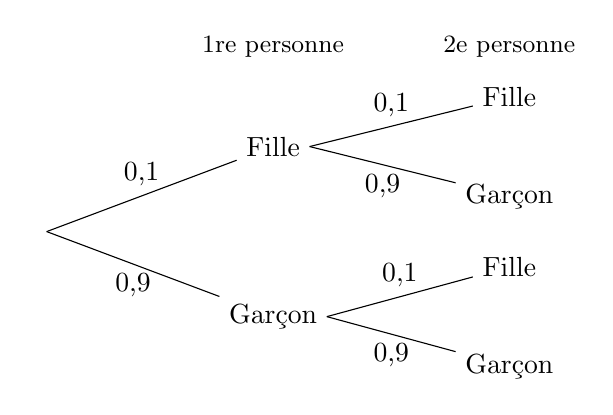
\begin{tikzpicture}[x=3cm, y=0.9cm]
		
		\node (root) at (0,0) {};
		\node (F) at (1,1.2) {Fille};
		\node (G) at (1,-1.2) {Garçon};
		\node (F1) at (2,1.9) {Fille};
		\node (G1) at (2,0.5) {Garçon};
		\node (F2) at (2,-0.5) {Fille};
		\node (G2) at (2,-1.9) {Garçon};
		
		\draw (root.east) -- (F) node[pos=0.5,above] {0,1};
		\draw (root.east) -- (G) node[pos=0.5,below] {0,9};
		
		\draw (F.east) -- (F1) node[pos=0.5,above] {0,1};
		\draw (F.east) -- (G1) node[pos=0.5,below] {0,9};
		\draw (G.east) -- (F2) node[pos=0.5,above] {0,1};
		\draw (G.east) -- (G2) node[pos=0.5,below] {0,9};
		
		\node at (1,2.6) {\small 1\up{re} personne};
		\node at (2,2.6) {\small 2\up{e} personne};
	\end{tikzpicture}
\end{center}

Les choix étant indépendants :
\[P(\text{deux garçons}) = 0,9 \times 0,9 = 0,81.\]

La probabilité que l’on choisisse deux garçons est égale à $0,81$.
